\documentclass[sigconf,balance]{acmart}
\usepackage[utf8]{inputenc}
\usepackage{multicol}
\usepackage{multirow}
\usepackage{amsmath}
\usepackage{amssymb}
\usepackage{xinttools}
\usepackage{array}
\usepackage{booktabs} % For formal tables
\usepackage{pgf, tikz}
\usepackage{pgfplots}

% for backwards compatibility
\usepackage{graphicx}

\usetikzlibrary{calc}

\setcopyright{rightsretained}
\newtheorem{theorem}{Theorem}

% DOI
\acmDOI{}

% ISBN
\acmISBN{}

% Conference
\acmConference[PCSC2019]{Philippine Computing Science Congress}{March 2019}{City of Manila, Philippines}
\acmYear{2019}

\acmArticle{}
\acmPrice{}

% These commands are optional
%\acmBooktitle{Transactions of the ACM Woodstock conference}
% \editor{}
% \editor{}
% \editor{}


\begin{document}
\title{Privacy-Preserving Approximation of Transcendental Functions}

\author{Aldrich Ellis C. Asuncion}
\affiliation{%
  % \department{Department of Information Systems and Computer Science}
  \institution{Ateneo de Manila University}
  \streetaddress{Katipunan Avenue, Loyola Heights}
  \city{Quezon City}  
  \country{Philippines}
  \postcode{1108}
}
\email{aldrich.asuncion@obf.ateneo.edu}

\author{Brian Christopher T. Guadalupe}
\affiliation{%
  % \department{Department of Information Systems and Computer Science}
  \institution{Ateneo de Manila University}
  \streetaddress{Katipunan Avenue, Loyola Heights}
  \city{Quezon City}
  \country{Philippines}
  \postcode{1108}
}
\email{brian.guadalupe@obf.ateneo.edu}

\author{William Emmanuel S. Yu}
\affiliation{%
  % \department{Department of Information Systems and Computer Science}
  \institution{Ateneo de Manila University}
  \streetaddress{Katipunan Avenue, Loyola Heights}
  \city{Quezon City}
  \country{Philippines}
  \postcode{1108}
}
\email{wyu@ateneo.edu}

% \maketitle
% The default list of authors is too long for headers.
\renewcommand{\shortauthors}{A. Asuncion, B. Guadalupe, and W. Yu}

\begin{abstract}
\begin{thesisabstract}
    \noindent
    Homomorphic cryptography allows for encrypted data to be modified and operated on without requiring decryption, although current homomorphic cryptosystems are either limited in their permitted operations or are significantly more time-intensive than standard non-homomorphic cryptosystems. Regardless, homomorphic cryptography has been targeted for use in secure image processing and facial recognition, due to their ability to maintain data privacy. In this paper, we compared the viability of the Paillier, Damg{\aa}rd--Geisler--Kr{\o}igaard (DGK), and Brakerski--Gentry--Vaikuntanathan (BGV) cryptosystems for facial image processing applications, by implementing a software library equipped with these cryptosystems, and comparing their time efficiency and accuracy. Furthermore, as an extension to previous research, we attempt to support non-linear image processing operations by deriving and implementing applicable closed-form approximations. Preliminary results have shown that the Paillier and DGK cryptosystems are comparable in accuracy and may be used for image negation, but only the Paillier cryptosystem is consistent enough to produce reasonable to accurate results.

    % This paper is a sample document that serves as a format and content guideline for undergraduate thesis submissions to the Department of Information Systems and Computer Science. In this section, the abstract, the group should be able to give the readers a clear and concise overview of their study. The section should contain the objectives of the thesis, the methods to be used, and when available, the results of the study, the conclusion, and the recommendations for further work, all based on the intended research objectives. A good abstract should be at most around 150--200 words, or half a page. It should also not contain any references, figures, or equations.
\end{thesisabstract}

\end{abstract}

%
% The code below should be generated by the tool at
% http://dl.acm.org/ccs.cfm
% Please copy and paste the code instead of the example below.
%
\begin{CCSXML}
    <ccs2012>
    <concept>
    <concept_id>10002950.10003714.10003736.10003737</concept_id>
    <concept_desc>Mathematics of computing~Approximation</concept_desc>
    <concept_significance>500</concept_significance>
    </concept>
    <concept>
    <concept_id>10002950.10003714.10003740</concept_id>
    <concept_desc>Mathematics of computing~Quadrature</concept_desc>
    <concept_significance>500</concept_significance>
    </concept>
    <concept>
    <concept_id>10002978.10002991.10002995</concept_id>
    <concept_desc>Security and privacy~Privacy-preserving protocols</concept_desc>
    <concept_significance>500</concept_significance>
    </concept>
    <concept>
    <concept_id>10002978.10002979.10002981.10011745</concept_id>
    <concept_desc>Security and privacy~Public key encryption</concept_desc>
    <concept_significance>300</concept_significance>
    </concept>
    </ccs2012>
\end{CCSXML}

\ccsdesc[500]{Mathematics of computing~Approximation}
\ccsdesc[500]{Mathematics of computing~Quadrature}
\ccsdesc[500]{Security and privacy~Privacy-preserving protocols}
\ccsdesc[300]{Security and privacy~Public key encryption}

\keywords{numerical methods; Gauss--Legendre quadrature; floating-point arithmetic; transcendental functions; homomorphic encryption; secure computation; Paillier cryptosystem}
% \keywords{cryptography; homomorphic encryption; data privacy; image processing; intensity transformation; facial recognition; numerical approximations}

\maketitle

\section{Introduction}
\subsection{Context of the Study}
Digital data privacy and security is a growing concern in various fields, such as cloud computing~\cite{potey_homomorphic_2016}, health information systems~\cite{kester_cryptographic_2015}, and video surveillance~\cite{upmanyu_efficient_2009}. To meet these needs, various cryptosystems have been developed. A cryptosystem is a system which operates on plaintexts, ciphertexts and keys using an encryption algorithm, which maps a plaintext to a ciphertext, together with a decryption algorithm, which maps a ciphertext to a plaintext, given an appropriate key~\cite{bauer_cryptosystem_2005}. The encryption and decryption algorithms are chosen such that the plaintext cannot easily be recovered from the ciphertext without knowledge of the key. This allows data to be securely transmitted over an insecure channel. Much research has been done on the development and application of various cryptosystems.

One particular application of cryptography is image encryption. While cryptosystems used to encrypt digital data in general, such as the Advanced Encryption Standard (AES) or elliptic curve cryptography, can also be used to encrypt images~\cite{jain_image_2016, singh_image_2015} other algorithms created specifically for image encryption have also been developed~\cite{murugan_survey_2018}.

In a homomorphic cryptosystem, operations such as addition and multiplication can be performed on encrypted data. These operations are then preserved when the data is decrypted. In this manner, data is manipulated without compromising data privacy, as the encrypted data being operated on remains secure~\cite{fontaine_survey_2007, sen_homomorphic_2013}. While numerous homomorphic cryptosystems exist for use with digital data in general, in the area of homomorphic image encryption, there is additional interest in being able to perform image manipulation operations on the encrypted data such as image adjustment, filtering, and morphological/feature extraction operations~\cite{ziad_cryptoimg:_2016, gonzalez_digital_2008}. More advanced operations have also been implemented using homomorphic cryptosystems, such as facial recognition \cite{hutchison_privacy-preserving_2009} and neural networks \cite{hesamifard_cryptodl:_2017}. This study in particular focuses on facial recognition.

\subsection{Research Questions}
By implementing homomorphic cryptosystems and creating a library so they can be easily used, we aim to address our main research question: What is the best method for facial image data to be encrypted and manipulated for practical applications?

More specifically, our research will address the following sub-questions:
\begin{enumerate}
	\item Which homomorphic cryptosystems admit more image processing operations? How can existing homomorphic cryptosystems be modified to admit more image processing operations?
	\item Which homomorphic cryptosystems are the most time-efficient and the most accurate in applying image processing operations?
	\item Which homomorphic cryptosystems best preserve image quality in applying image processing operations?
\end{enumerate}


\subsection{Research Objectives}
Previous attempts in the literature to provide image processing tasks such as image manipulation \cite{ziad_cryptoimg:_2016} and  facial recognition \cite{hutchison_privacy-preserving_2009} have primarily used the Paillier and  Damg{\aa}rd--Geisler--Kr{\o}igaard (DGK) cryptosystems to perform linear operations on encrypted data. In this study, we extend this research to provide an objective comparison of various homomorphic cryptosystems currently in the literature in performing non-linear operations, as opposed to just linear operations, and facial detection, as opposed to just facial recognition.

Our main research objective is to assess the practicality of various homomorphic cryptosystems with regard to image processing on faces. Homomorphic cryptosystems are known to be slower in terms of encryption, operation, and decryption time~\cite{sen_homomorphic_2013}. Furthermore, the operations on encrypted data supported by homomorphic cryptosystems are limited, and some schemes require preprocessing to be performed on images, limiting the range of operations which can be performed efficiently~\cite{li_elliptic_2012}.

In summary, in this study, we wish to
\begin{enumerate}
    \item Implement common image processing operations using known homomorphic encryption schemes, then determine which schemes admit more image processing operations and extend known cryptosystems to support more operations, if possible;
    \item Compare the time efficiency and accuracy of common image processing operations under known homomorphic encryption schemes, and of common image processing operations without using homomorphic encryption;
    \item Create a library to allow for convenient use and comparison of these homomorphic encryption schemes for image processing and facial recognition.
\end{enumerate}

\subsection{Scope and Limitations}
Our study will be limited in terms of the cryptosystems to be tested, the image processing operations we will implement, and the statistical tests we will use to gauge the security of the cryptosystems. Below is a listing of the scope of the study.

We will implement and test the following algorithms:
\begin{enumerate}
	\item A variant of the Paillier cryptosystem~\cite{stern_public-key_1999} which supports floating-point operations, used in \textit{CryptoImg}~\cite{ziad_cryptoimg:_2016}.
    \item The Damg{\aa}rd--Geisler--Kr{\o}igaard (DGK) cryptosystem~\cite{pieprzyk_efficient_2007, cryptoeprint:2008:321} which is primarily used for secure integer comparison.
	\item A fully homomorphic encryption scheme by Dasgupta and Pal, which uses polynomial rings~\cite{dasgupta_design_2016}.
	\item The Brakerski--Gentry--Vaikuntanathan (BGV) cryptosystem \cite{cryptoeprint:2011:277}, an improvement on the lattice-based cryptosystem by Gentry~\cite{gentry_fully_2009}, with optimizations from Smart, Vercauteren, and Halevi \cite{hutchison_fully_2010, cryptoeprint:2011:566}.
\end{enumerate}
We will implement and test the following categories of image manipulation operations:
\begin{enumerate}
	\item Non-linear image intensity adjustment (logarithm and power-log transformations)
	\item Facial detection and recognition using the eigenface approach \cite{turk_eigenfaces_1991}.
\end{enumerate}
We will adopt the benchmark for evaluating image quality of image encryption schemes presented by Ahmed, et. al~\cite{ahmed_benchmark_2016}. The presented benchmark reflects many tests used in other literature~\cite{ahmad_efficiency_2012, wu_npcr_2011}.
\begin{enumerate}
    \item Mean Squared Error (MSE)
    \item Peak Signal to Noise Ratio (PSNR)
    \item Structural Similarity Index (SSIM)
\end{enumerate}
A detailed overview of the above will be provided in the methodology. Grayscale images will be used in the study.
A client-server model for secure computation will be assumed to allow operations such as secure comparison and exponentiation.
Training and test data are taken from the publicly available \texttt{faces94} dataset (\url{https://cswww.essex.ac.uk/mv/allfaces/faces94.html}) maintained by the University of Essex. 

\subsection{Significance of the Study}
This study aims to directly address one of the current problems in the research of homomorphic cryptosystems: the practicality of homomorphic encryption~\cite{sen_homomorphic_2013}. The literature shows existing homomorphic cryptosystems and how they support primitive operations (usually addition and multiplication) on encrypted data, however, for homomorphic cryptosystems to be useful for practical use, efficient support for more complicated image processing operation must be demonstrated as well. While implementations of image processing operations in a homomorphic cryptosystem exist in the literature~\cite{ziad_cryptoimg:_2016, garay_algorithms_2014}, our study targets the more computationally intensive task of facial detection.

We wish to contribute to existing models for the secure transmission and modification of image data by developing a software library which allows the use and comparison of various homomorphic encryption algorithms. Our software library would allow service providers to perform image manipulation for clients without compromising data privacy.


\section{Review of Related Literature}
\subsection{Homomorphic Cryptosystems}
A cryptosystem consists of an encryption function $\mathcal{E}$ and a decryption function $\mathcal{D}$, along with the plaintext space $\mathcal{P}$, ciphertext space $\mathcal{C}$ and the key space $\mathcal{K}$~\cite{bauer_cryptosystem_2005}. A \textit{plaintext} is text that can be commonly understood, while a \textit{ciphertext} results from encrypting the plaintext using an encryption key. The \textit{plaintext space} is the set of all possible plaintexts, the \textit{ciphertext space} is the set of all possible ciphertexts, while the \textit{keyspace} is the set of all possible keys.

There are two kinds of cryptosystems, \textit{symmetric} and \textit{asymmetric}. In symmetric-key cryptosystems, the same key is used for both encryption and decryption. As a consequence, symmetric-key cryptosystems must be implemented with a secure key exchange protocol, so that both the sender and receiver have access to the same key. Prominent examples of symmetric-key cryptosystems are the Data Encryption Standard (DES), and its replacement, the Advanced Encryption Standard (AES).

On the other hand, asymmetric-key (or public-key) cryptosystems use separate keys for encryption and decryption. The encryption key (also called the \textit{public key}) is shared publicly, while the decryption key (also called the \textit{private key}) is kept secret. Since the public key and private keys are different, there is no need to agree upon secure key exchange protocols. Usually, the security of asymmetric-key cryptosystems relies on the intractability of certain computational problems, for example, the RSA cryptosystem depends on the difficulty of big integer factorization~\cite{rivest_method_1978}, while the ElGamal cryptosystem depends on the difficulty of the discrete logarithm problem~\cite{blakley_public_1985}.

Homomorphic cryptosystems are a special type of cryptosystem in which operations can be securely performed on encrypted data. Suppose that for a public-key cryptosystem, $\mathcal{E}_k \left(p \right)$ is the encryption function using the public key $k \in \mathcal{K}$, and $\mathcal{D}_l \left(c \right)$ be the decryption function using the private key $l$. A cryptosystem is said to be homomorphic if its encryption function is homomorphic, that is, if it satisfies the relation
\begin{equation}
    \mathcal{E}_k \left(p_1 \boxplus p_2\right) = \mathcal{E}_k \left(p_1\right) \boxdot \mathcal{E}_k \left(p_2\right)
\end{equation}
where $p_1, p_2 \in \mathcal{P}$ are the plaintexts, and $\boxplus$ and $\boxdot$ are operations in $\mathcal{P}$ and $\mathcal{C}$ respectively~\cite{fontaine_survey_2007}. Furthermore, a homomorphic cryptosystem also satisfies~\cite{li_elliptic_2012}
\begin{equation}
    p_1 \boxplus p_2 = \mathcal{D}_l \left( \mathcal{E}_k \left(p_1\right) \boxdot \mathcal{E}_k \left(p_2\right) \right).
\end{equation}
In other words, a homomorphic cryptosystem preserves the operations that can be done with the plaintext without requiring an intermediary step of decrypting the ciphertext beforehand. It is important to note that the operations $\boxplus$ and $\boxdot$ need not be the same. A simple operation in the plaintext space may require a computationally intensive operation in the ciphertext space.

Homomorphic cryptosystems can be classified according to the plaintext and ciphertext operations, $\boxplus$ and $\boxdot$. If the plaintext operation $\boxplus$ is addition, the cryptosystem is said to be \textit{additively homomorphic}, and the cryptosystem is said to be \textit{multiplicatively homomorphic} if the plaintext operation $\boxplus$ is multiplication.

\subsection{Partially Homomorphic Cryptosystems}
In this section, we will present two classical partially homomorphic cryptosystems which we will be testing in the study: the Paillier cryptosystem and the DGK cryptosystem. Both of these cryptosystems encrypt integer plaintexts and are additively homomorphic.

We will then show that the cryptosystems can be modified to support privacy-perserving polynomial evaluation in a client-server protocol: given an encrypted message $m$, evaluate $f(m)$ where $f$ is a polynomial function.

\subsubsection{The Paillier Cryptosystem}
The Paillier cryptosystem \cite{stern_public-key_1999}, developed by Pascal Paillier, is a probabilistic encryption scheme which is based on the composite residuosity class problem. The scheme allows for the encryption and decryption of integer messages, and is known to be additively homomorphic. We now state the encryption and decryption algorithms of the Paillier cryptosystem and its homomorphic properties.

\paragraph{Key Generation}
We first define a function $L(x)$ as the largest integer $v$ greater than zero such that $x-1 \geq vn$.
We choose two large primes $p$ and $q$, and set $n = pq, \lambda = \mathrm{lcm}(p-1,q-1)$.
Then we select an integer $g$, $0\leq g \leq n^2$ such that $\mathrm{gcd}(L(g^\lambda \bmod n^2), n) = 1$.
We denote the public key as $(g,n)$ and the private key $(p,q)$.

\paragraph{Encryption and Decryption}
The encryption function to encrypt a plaintext $m \in \mathbb{Z}_n$ given a public key $(g,n)$ is defined as
\begin{align*}
  E(m) = g^m \cdot r^n \mod{n^2},
\end{align*}
where $r$ is a random non-negative integer less than $n^2$.

The decryption function to decrypt a ciphertext $c \in \mathbb{Z}^\ast_{n^2}$ given a private key $(p,q)$ is defined as:
\begin{align*}
  D(c) = L(c^\lambda \bmod n^2) \times (L(g^\lambda \bmod n^2))^{-1} \mod n
\end{align*}

\paragraph{Homomorphic Properties of the Paillier Cryptosystem}
The Paillier cryptosystem supports additive homomorphism as well as the multiplication of a plaintext scalar to an encrypted message. These homomorphic properties are used to add a plaintext scalar to a ciphertext, add two ciphertexts, and multiply a ciphertext by a plaintext scalar, respectively. They are defined as follows.

For all $m_1,m_2 \in \mathbb{Z}_n$ and $k\in \mathbb{N}$, the following homomorphic properties hold.
\begin{align*}
  D(E(m_1)g^k\bmod n^2) &=(m_1+k)\bmod n\\
  D(E(m_1)E(m_2)\bmod n^2) &=(m_1+m_2)\bmod n\\
  D(E(m_1)^k\bmod n^2) &= km_1\bmod n
\end{align*}

\subsubsection{The DGK Cryptosystem}
The DGK cryptosystem was published by Damg{\aa}rd, Geisler, and Kr{\o}igaard in 2007 in an effort to create a secure integer comparison scheme \cite{pieprzyk_efficient_2007, cryptoeprint:2008:321} which is widely used in the literature \cite{veugen_improving_2012}.

\paragraph{Key Generation}
We denote $k,t,\ell$ as security parameters of the scheme, where $k>t>\ell$.
Let $p,q$ be primes such that
we can choose two $t$-bit primes $v_p$ and $v_q$ such that $v_p | (p-1)$ and $v_q | (q-1)$, and a small prime $u$ such that $u | (p-1)$ and $u | (q-1)$.
We denote $n = pq$.
We choose $g$ to be an integer of order $uv_pv_q$ and $h$ to be of order $v_pv_q$.

The DGK cryptosystem encrypts plaintexts in $\mathbb{Z}_u$ to ciphertexts in $\mathbb{Z}_n^\ast$.

The public key is $(n,g,h,u)$ and the private key is $(p,q,v_p,v_q)$.

\paragraph{Encryption and Decryption}
To encrypt a message $m \in \mathbb{Z}_u$, the encryption function is defined as:
\begin{align*}
  E(m) = g^m \cdot h^r \mod{n},
\end{align*}
where $r$ is a random integer in $\mathbb{Z}_n$ which is longer than $2t$ bits.

To decrypt a ciphertext $c \in \mathbb{Z}_n^\ast$, decryption is achieved by first computing $c^{v_pv_q}$.
\begin{align*}
	c^{v_pv_q} \bmod n
	&= (g^m \cdot h^r)^{v_pv_q} \bmod n\\
	&= (g^{v_pv_q})^m \bmod n
\end{align*}
Since $(g^{v_pv_q})^m$ has order $u$, there is a one-to-one correspondence between plaintexts in $\mathbb{Z}_u$ and  $(g^{v_pv_q})^m$. A lookup table can thus be generated privately to successfully recover $m$.

\paragraph{Homomorphic Properties of the DGK Cryptosystem}
The DGK cryptosystem supports additive homomorphism as well as the multiplication of a plaintext scalar to an encrypted message. These homomorphic properties are used to add a plaintext scalar to a ciphertext, add two ciphertexts, and multiply a ciphertext by a plaintext scalar, respectively. They are defined as follows.

For all $m_1,m_2 \in \mathbb{Z}_u$ and $k\in \mathbb{N}$, the following homomorphic properties hold.
\begin{align*}
    D(E(m_1)g^k) &=(m_1+k)\bmod u\\
    D(E(m_1)E(m_2)) &=(m_1+m_2)\bmod u\\
    D(E(m_1)^k) &= km_1\bmod u
\end{align*}

As the multiplicative homomorphism was not presented in the original paper, we provide a short proof here.
\begin{proof}
  Let $m \in \mathbb{Z}_u$ and $k\in \mathbb{N}$.
  We consider $E(m)^k = (g^m \cdot h^r \bmod{n})^k\bmod n$.
  \begin{align*}
    (g^m \cdot h^r \bmod{n})^k \bmod n
    &= (g^m \cdot h^r)^k \bmod{n}\\
    &= (g^m)^k \cdot (h^r)^k \bmod{n}\\
    &= g^{km} \cdot (h^kr) \bmod{n}\\
  \end{align*}
  Since $r$ is a random integer, $kr$ is also a random integer, Therefore, $g^{km} \cdot (h^kr) \bmod{n} = D(E(m_1)^k)$ is a valid encryption of the message $km$.
\end{proof}


\subsubsection{Secure Exponentiation and Multiplication Protocols}
\label{ssec:exponentiationprotocol}
In order to perform polynomial evaluation, we first present a protocol for privacy-preserving exponentiation to a positive integer power, adapted from the protocol to calculate Euclidean distances used in \cite{hutchison_privacy-preserving_2009}.

The following protocols apply to both the Paillier and DGK cryptosystems, as they share similar homomorphisms. We first present a secure squaring protocol.

Suppose Alice encrypts an integer $x$ and sends it so Bob has $E(x)$, and wants to obtain $E(x^2)$ without exposing the value of $x$.
\begin{itemize}
	\item Bob first selects a random integer $r$ and computes $E(x+r)$. Bob can do this since $r$ is a plaintext constant.
	\item Bob sends $E(x+r)$ to Alice, who decrypts the ciphertext to obtain $x+r$.
	\item Alice squares $x+r$ and encrypts the result. She sends $E((x+r)^2)$ to Bob.
	\item Bob computes $E(-2rx + r^2)$. He then computes $E((x+r)^2)E(-2rx + r^2) = E(x^2)$.
\end{itemize}

We can use the secure squaring protocol to arrive at a secure multiplication protocol, which then allows for the evaluation of polynomials.
Suppose Alice encrypts integers $x$ and $y$, and Bob has $E(x), E(y)$ and wants to obtain $E(xy)$.
\begin{itemize}
	\item Bob acquires $E(x^2), E(y^2)$ using the secure squaring protocol.
	\item Bob sends $E(x+y)$ to Alice, who decrypts the ciphertext to obtain $x+y$.
	\item Alice sends $E((x+y)^2)$ to Bob.
	\item Bob then computes
	\begin{align*}
		E((x+y)^2)E(x^2)^{-1}E(y^2)^{-1} &= E((x+y)^2 - x^2 - y^2)\\
		&= E(2xy)
	\end{align*}
	\item Bob can then recover $E(xy)$ by calcuating for the multiplicative inverse of 2 using the Euclidean algorithm, and calculating $2^{-1}E(xy)$. Such an inverse exists since the modulus is either a prime (in the DGK cryptosystem) or a product of primes greater than 2 (in the Paillier cryptosystem).
\end{itemize}

\subsection{Fully Homomorphic Cryptosystems}
We will also be testing fully homomorphic cryptosytems, which allow aribitrary computation on encrypted data.
While generally being more flexible, fully homomorphic cryptosytems are known to be significantly slower than partially homomorphic cryptosytems; improving the efficiency of fully homomorphic cryptosytems is an active area of research \cite{sen_homomorphic_2013}.

We will present two such cryptosystems, the Dasgupta--Pal cryptosystem, which we present in full to explain a correction we propose to it, and the BGV cryptosystem, which has open source implementations availble primarily used in homomorphic cryptography research.

\subsubsection{The Dasgupta--Pal Cryptosystem}
The Dasgupta--Pal cryptosystem is a fully homomorphic cryptosystem proposed in 2016 by Smaranika Dasgupta and S. K. Pal \cite{dasgupta_design_2016}, which encrypts integer plaintexts in $\mathbb{Z}_n$ to polynomial ciphertexts. We begin our presentation of the Dasgupta--Pal cryptosystem with the following definition.

Given a message $m \in \mathbb{Z}$, we denote
\begin{align*}
		m_p(x) = a_0 + a_1 x + a_2 x^2 + \cdots + a_k x^k
\end{align*}
where $a_k a_{k-1}\cdots a_2 a_1 a_0$ is the binary representation of $m$.

In the original scheme presented in \cite{dasgupta_design_2016}, the secret key $S_k$ is set to be a large prime. In Appendix \ref{chap:correction}, we present a case where the Dasgupta--Pal cryptosystem fails and prove that setting the secret key $S_k = 2p$, where $p$ is a large prime, corrects errors in the Dasgupta--Pal cryptosystem.
We now decribe the correct cryptosystem.
\paragraph{Corrected Dasgupta--Pal Cryptosystem Description}
Let $\ell$ denote the security parameter of the cryptosystem.
Let $S_k = 2p$, where $p$ is a prime number with $\ell - 1$ bits.
Choose a random even integer $z$ of length $\log_2{\ell}$.

Let the secret key be $S_k$, and let the refresh key be $R_k = z \cdot S_k$. The secret key is kept private to the encrypting/decrypting parties, while the refresh key is made publicly available.

The scheme defines the encryption algorithm for a message $m$ as follows:
\begin{align*}
	E(m) = y(x) + S_k\times d(x)
\end{align*}
where
$y(x)$ is a polynomial of degree $n$ such that $m_p(x) \equiv y(x) \bmod S_k$ and $d(x)$ is a randomly chosen polynomial of degree $n$. This encrypts each coefficient of $m_p(x)$ by adding some multiple of $S_k$ to it. Through this process, each bit of the message is encrypted separately.

Furthermore, the decryption algorithm to recover $m_p(x)$ from a ciphertext polynomial $c(x)$ as
\begin{align*}
	m_p(x) = c(x) \bmod S_k \bmod 2.
\end{align*}
Thus $D(c(x))$ is defined as the integer recovered from the coefficients of the polynomial $c(x) \bmod S_k \bmod 2$.

Dasgupta and Pal note that homomorphic operations on ciphertext introduce noise which may interfere with decryption, due to the potential increase in ciphertext values.
To eliminate noise from a polynomial ciphertext, the following refresh function is used:
\begin{align*}
	R(c(x)) = c(x) \bmod R_k.
\end{align*}

\paragraph{Homomorphic Properties of the Dasgupta--Pal Cryptosystem}
It has been shown \cite{dasgupta_design_2016} that the following properties hold for all integer messages $m_1, m_2 \in \mathbb{Z}_n$ in the Dasgupta--Pal cryptosystem. These properties arise since each coefficient in a ciphertext polynomial is essentially an independently encrypted bit of the original message.
\begin{description}
	\item[\textsc{xor} on ciphertexts]
	A bitwise exclusive or (\textsc{xor}) operation on integer messages can be achieved by adding the coefficients pairwise between two ciphertexts.
	\begin{align*}
		D(E(m_1)+E(m_2)) = m_1 \textsc{ xor } m_2
	\end{align*}
	\item[\textsc{and} on ciphertexts]
	Similarly, pair-wise multiplication corresponds to bitwise \textsc{and} of integer messages.
	\begin{align*}
		D(E(a) \otimes E(b)) = a \textsc{ and } b = ab \bmod 2
	\end{align*}
	where $\otimes$ denotes pairwise multiplication,
	\begin{align*}
		\sum_{i=1}^n{a_ix^i} \otimes \sum_{i=1}^n{b_ix^i} = \sum_{i=1}^n{a_ib_ix^i}.
	\end{align*}
\end{description}

Arbitrary computation on data can thus be achived using these bitwise operations. While the Dasgupta--Pal cryptosystem requires significant amounts of memory, as each bit of plaintext is encrypted into an integer, this approach provides a flexible method to perform relatively fast arbitrary computation on encrypted data. Encryption and decryption in the Dasgupta--Pal cryptosystem are accomplished using few arithmetic operations.

\subsubsection{HElib and the BGV Cryptosystem}
The BGV (Brakerski--Gentry--Vaikuntanathan) cryptosystem \cite{cryptoeprint:2011:277} is a fully homomorphic cryptosystem created based on the ring-learning with error problem. The BGV cryptosystem was constructed to surpass the limitations of prior fully homomorphic cryptosystems, which were based on the first fully homomorphic cryptosystem by Gentry \cite{gentry_fully_2009}.

The details regarding the construction of the BGV cryptosystem are beyond the scope of this paper. For this study, we will be using \textit{HElib} \cite{garay_algorithms_2014}, an open-source library which implements the BGV cryptosystem with optimizations to improve efficiency. Evaluation of operations on 120 inputs in HELib was performed in around 4 minutes, with an average of 2 seconds to process a single input \cite{hutchison_fully_2010,cryptoeprint:2011:566}.

The \textit{HElib} library has been adapted to Python using the Pyfhel library \cite{pyfhel_2018} maintained by Ibarrondo, Laurent (SAP) and Onen (EURECOM), and licensed under the GNU GPL v3 license. The Pyfhel library is a Python API for the \textit{HElib} library, which supports the following operations on vectors/scalars of integers or binary ciphertexts:
\begin{itemize}
	\item Arithmetic operations: addition, subtraction, multiplication;
	\item Binary operations: \textsc{and}, \textsc{or}, \textsc{not}, \textsc{xor}.
\end{itemize}

\subsection{CryptoImg}
A paper published in 2009 by Ziad, et al. attempts to implement privacy-preserving image processing using \textit{CryptoImg}, a library for the Open Source Computer Vision Library (OpenCV)~\cite{bradski_opencv_2000} which implements various homomorphic encryption and image processing routines using the Paillier homomorphic cryptosystem~\cite{ziad_cryptoimg:_2016}. The CryptoImg library assumed a client-server model wherein a client requests image processing operations from a server. A client first encrypts a digital image and sends the image securely to a server, which then operates on the encrypted image without revealing its contents. Then the resulting image is sent back to the client, which decrypts the image to recover the desired output.
\begin{figure}[!ht]
    \centering
    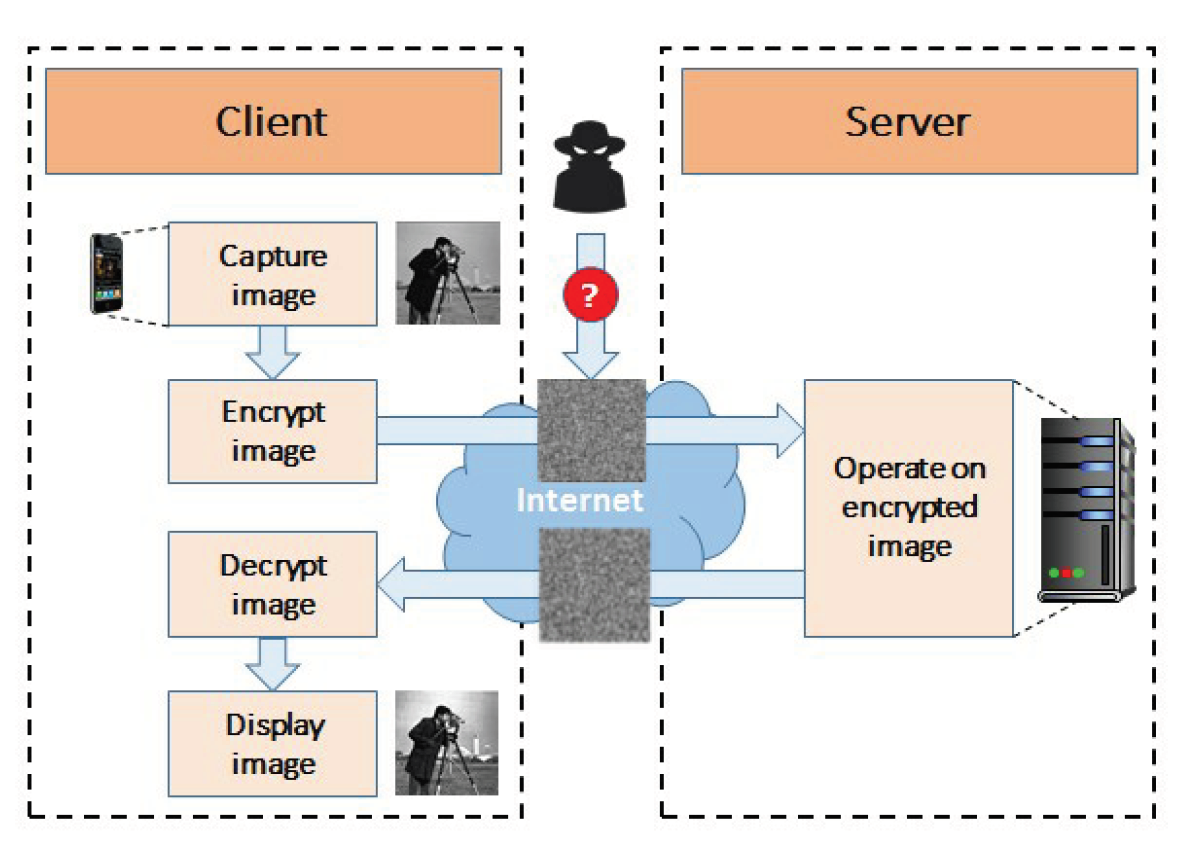
\includegraphics[width=0.4\textwidth]{figures/ClientServerModel.png}
    \caption{Client-server architecture used by \textit{CryptoImg} \cite{ziad_cryptoimg:_2016}}
    \label{fig:clientserver}
\end{figure}

The \textit{CryptoImg} library implemented the following:
\begin{enumerate}
	\item Extending the Paillier homomorphic cryptosystem which operate on integer plaintexts so that they can operate on real number plaintexts;
	\item Developing protocols for and implementing the following image processing operations
	\begin{enumerate}
		\item Image negation and brightness adjustment
		\item Spatial filters (for noise reduction, edge detection and sharpening)
		\item Morphological operations
		\item Histogram equalization
	\end{enumerate}
\end{enumerate}
For image negation and spatial filters, the protocols specified by \textit{CryptoImg} allow all image processing operations to be performed on the server. However, due to limitations in the Paillier cryptosystem, the protocols presented for morphological operations and histogram equalization require both the client and the server to perform image processing calculations, although the server performs a significant portion of the processing.

Ziad, et al. also showed experimental results establishing the slow performance of image operations under a homomorphic cryptosystem. For instance, while sharpening and applying a Sobel filter each take less than a second when applied to a $512\times 512$ plaintext image, when applied to an encrypted image, sharpening required at least 238.257 seconds, and applying the Sobel filter required at least 147.567 seconds \cite{ziad_cryptoimg:_2016}.

We now discuss several limitations in the \textit{CryptoImg} study which we focus on for our research. First, the \textit{CryptoImg} library was limited in the image intensity transformations it implemented. We propose additional protocols to support more computationally intensive intensity transformations.
Second, the \textit{CryptoImg} library only considered the Paillier cryptosystem. We consider testing the performance of other homomorphic cryptosystems, which differ in their processing time and supported operations.

\subsection{Image Intensity Transformations}
We represent a digital image $R$ as an $M \times N$ matrix of pixel intensity values, each value in the range $\left[0, L-1\right]$, for some positive integer $L$. We use $R(x,y)$ to represent the entry at the $x$th row and $y$th column of a matrix $R$.
An intensity transformation on an image $R$ can be defined as a function $T$ which maps a pixel value $r$ to a new value $r^\prime$, which we can write as $r^\prime = T\left(r\right)$. This function is then applied to every pixel in $R$.
The \textit{CryptoImg} library implemented two types of linear intensity transformations: image negation and brightness control.

An image negation transformation is defined as:
\begin{equation}
    T\left(r\right) = L-1-r
\end{equation}
After applying image negation, the resulting image would be similar to a photographic negative~\cite{gonzalez_digital_2008}.

A brightness control transformation with parameter $v$ is defined as:
\begin{equation}
    T\left(r,v\right) = r+v
\end{equation}
The above transformations are linear in terms of the input $r$, and are thus simple to implement under a homomorphic cryptosystem.

In this study we extend the range of intensity transformations to non-linear transformations. Two common non-linear image transformations are the log transformation and power-law transformation~\cite{gonzalez_digital_2008}.

The log transformation is used to enhance dark pixels or increase the dark details of an image by mapping low intensity values to a wider range of values~\cite{gonzalez_digital_2008}. This has the general formula
\begin{equation}
    T\left(r\right) = c \log\left(1 + r\right)
\end{equation}
where $c$ is a constant.

The power-law transformation is a family of transformations that have the form
\begin{equation}
    T\left(r\right) = c r^{\gamma}
\end{equation}
where $c>0$ and $\gamma > 0$.
A power-law transformation defined by the above equation can calibrate the operation of many image capture and output devices such as cameras, printers and displays in a process called \textit{gamma correction}. This ensures reproducibility and accuracy of images being displayed by digital output devices~\cite{gonzalez_digital_2008}.

To implement non-linear intensity transformations using addition and multiplication in a homomorphic system, it is necessary to approximate the logarithm and exponential functions, which may result in higher computational overhead. In our software library implementation, we investigate methods required to approximate the logarithm and power functions. Non-linear intensity transformations such as the logarithm transformation have applications in intensity normalization \cite{oravec_illumination_2010}, which is used in some facial recognition algorithms to account for differences in lighting which make facial recognition difficult.

\subsection{Facial Detection and Recognition}
%% TODO: Brian dump ur stuff here

Since simple image operations mentioned earlier can be done within a homomorphic cryptosystem, these operations can be assembled together in order to do more complex operations. A prominent application of image processing that often uses complex image operations is \textit{facial recognition}.

Traditional facial recognition algorithms rely on detecting salient features in a face image. One of the popular facial recognition algorithms is \textit{eigenfaces}.
% Traditional facial recognition algorithms rely on detecting salient features in a face image. Two of the popular facial recognition algorithms are \textit{eigenfaces} and \textit{Haar cascades}.

\subsubsection{Eigenfaces}
Proposed by Matthew Turk and Alex Pentland, the eigenfaces method uses principal component analysis (PCA) in order to express an input image as a linear combination of eigenfaces \cite{turk_eigenfaces_1991}. An \textit{eigenface} is a principal component, or more simply an eigenvector that represents a certain variation between the face images which are taken from the initial training set. The number of resulting eigenfaces is equal to the number of face images in the training set.

In the enrollment process, $M$ face images $\Theta_1, \ldots, \Theta_M$, each of size $p \times q$, are taken in to comprise the initial training set. The training images can be represented as vectors of length $N = pq$, where each row of an image is concatenated together.

The average of the training images, denoted as $\Psi$, is 
\begin{equation}
	\Psi = \frac{1}{M} \sum_{i=1}^{M} \Theta_i
\end{equation}

The \textit{difference vectors} are then computed as $\Phi_i = \Theta_i - \Psi$. PCA is applied on the covariance matrix of the vectors
\begin{equation}
	\mathbf{C} = \frac{1}{M} \sum_{i=1}^M \Phi_i \Phi_i^\top = \frac{1}{M} \mathbf{A}\mathbf{A}^\top,
\end{equation}
where $\mathbf{A}$ is an $N \times M$ matrix defined by $\left[\Theta_1 \quad \Theta_2 \quad \cdots \quad \Theta_M\right]$, in order to determine the orthonormal eigenvectors \cite{hutchison_privacy-preserving_2009}.

Directly computing the covariance matrix and then applying PCA will become inefficient for large sizes of $\mathbf{A}$, since computing for $\mathbf{A}\mathbf{A}^\top$ results in an $N \times N$ matrix, which can get drastically large because it is dependent on the size of the image. On the other hand, computing for $\mathbf{A}^\top\mathbf{A}$ only results in an $M \times M$ matrix, which is much smaller than the previous one because it is just dependent on the number of face images in the training set. Now, we can apply PCA to $\mathbf{A}^\top\mathbf{A}$ along with some post-processing to obtain the eigenvectors \cite{hutchison_privacy-preserving_2009}. 

Instead of getting the eigendecomposition of the covariance matrix by explicitly computing the eigenvalues and eigenvectors of $\mathbf{C}$, we can also apply \textit{singular value decomposition} (SVD) on the matrix $\Phi^\top$. This is because SVD works through a divide-and-conquer method which results in greater numerical stability, while eigendecomposition simply uses the traditional QR factorization \cite{nakatsukasa_stable_2013, gu_divide-and-conquer_1995}. Upon applying SVD, we now get the eigenvectors $\mathbf{u}_1, \ldots, \mathbf{u}_M$ and their corresponding eigenvalues $\lambda_1, \ldots, \lambda_M$.

We choose $K$ eigenvectors $\mathbf{u}_1, \ldots, \mathbf{u}_K$ such that it comprises a set associated with the $K$ largest eigenvalues, where $K$ is much smaller than $M$. This set is now the \textit{face space}. Then, the images $\Theta_1, \ldots, \Theta_K$ are projected onto the face space spanned by the eigenfaces to determine the weight vectors $\Omega_1, \ldots, \Omega_K$.

To perform the recognition process, the algorithm projects the input image $\Gamma$ onto the face space, and then comparing the projected image $\bar{\Omega} = \mathbf{u}_i\left(\Gamma - \Psi\right)$ with each eigenface in the face space using a metric such as the Euclidean distance. Thus it is computed as $d_i = \left\lVert \Omega_i -\bar{\Omega} \right\rVert$ for all $i=1,\ldots,K$, where $\left\lVert \cdot \right\rVert$ denotes the Euclidean norm.

Then, a match can be reported if the smallest possible distance is smaller than the given threshold value $T$. 
\newcommand{\argmin}{\mathop{\mathrm{arg\,min}}}  
\begin{equation}
	\text{ID} = \begin{cases}\argmin_i d_i & \text{if } \min_i d_i \le T \\\emptyset & \text {otherwise}\end{cases}
\end{equation}


\subsection{Previous Implementations of Secure Facial Recognition}
Erkin, et al. \cite{hutchison_privacy-preserving_2009} devised a method to incorporate the use of homomorphic cryptosystems into the eigenfaces method. In their study, they proposed a two-party system where Alice holds an encrypted image $\left[\Gamma\right]$, while Bob maintains a database of $K$ eigenfaces $\mathbf{u}_1, \ldots, \mathbf{u}_K$, and feature vectors $\Omega_1, \ldots, \Omega_M$ in the clear.

\begin{figure}[!h]
    \centering
    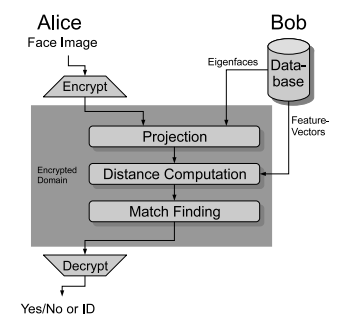
\includegraphics[width=0.4\textwidth]{figures/secure_eigenfaces.png}
    \caption{Diagram of the privacy-preserving facial recognition process \cite{hutchison_privacy-preserving_2009}}
\end{figure}


In order to ensure privacy, the steps in the eigenfaces algorithm, namely: projection, distance computation, and match finding, are done within the encrypted domain, i.e., using the operations in the Paillier cryptosystem.

Projection is similar to that of the original eigenfaces algorithm, except the operations are replaced with their respective operations in the cryptosystem. Distance computation in this version is somewhat different from the original eigenfaces method, in that it deals with the square of the Euclidean distance since the relative order of the distances is only important when comparing these during the match finding step \cite{hutchison_privacy-preserving_2009}.
\begin{align}
    d_i &= \left\lVert \Omega_i - \bar{\Omega} \right\rVert ^2 = \sum_{j=1}^{K} \left(\omega_{ij} - \bar{\omega}_j\right)^2 \\
        &= \underbrace{\sum_{j=1}^{K} \omega_{ij}^2}_{\mathcal{S}_1} + \underbrace{\sum_{j=1}^{K} \left(-2 \omega_{ij} \bar{\omega_j}\right)}_{\mathcal{S}_2} + \underbrace{\sum_{j=1}^{K} \bar{\omega}_{j}^2}_{\mathcal{S}_3}
\end{align}

Computing for the distances within Paillier would just be multiplying the encrypted sums together.
\begin{equation}
	\left[d_i\right] = \left[\mathcal{S}_1\right] \cdot \left[\mathcal{S}_2\right] \cdot \left[\mathcal{S}_3\right]
\end{equation}

The terms $\left[\mathcal{S}_1\right]$ and $\left[\mathcal{S}_2\right]$ can be easily computed by Bob, since he already knows both $\omega_i$ in the clear and $\left[\bar{\omega}_i\right]$ which is in encrypted form. Computing for $\left[\mathcal{S}_3\right]$ is trickier because Bob cannot compute for $\left[\bar{\omega}_i^2\right]$ because pairwise multiplication is not supported in Paillier, that is why Bob needs help from Alice to square a number through a protocol described below \cite{hutchison_privacy-preserving_2009}.

Before Bob sends $\left[\bar{\omega}_i\right]$ to Alice for squaring, he adds a random number $r_i$ to compute $\left[x_i\right] = \left[\bar{\omega}_i + r_i\right] = \left[\bar{\omega}_i\right] \cdot \left[r_i\right]$, where $r_i$ is obviously distinct for every $i$, then sends $\left[x_i\right]$ to Alice. She then decrypts it and computes $x_i^2$, and then computes $\mathcal{S}_3^\prime = \sum_{i=1}^{K} x_i^2$, after which she encrypts the sum and sends $\left[\mathcal{S}_3^\prime\right]$ to Bob. Now, he can compute for $\left[\mathcal{S}_3\right]$ as follows:
\begin{equation}
	\left[\mathcal{S}_3\right] = \left[\mathcal{S}_3^\prime\right] \cdot \prod_{j=1}^{K} \left(\left[\bar{\omega}_j\right]^{-2r_j} \cdot \left[-r_j^2\right]\right)
\end{equation}

The protocol for squaring a number as described earlier is a workaround for the limitations of Paillier or any other partially homomorphic cryptosystem that only supports addition and scalar multiplication. This can be possibly extended so that operations such as pairwise multiplication and exponentiation are also supported, provided that the protocol involves two parties.

The match finding step is done by comparing the distances obtained from the previous step to a specified threshold $T$. If the minimum distance is smaller than $T$, then a match is found, and the encrypted identity of the match is returned to Alice \cite{hutchison_privacy-preserving_2009}. Getting the minimum among the encrypted distances would involve comparing two encrypted numbers, which Paillier does not support. Instead, the DGK cryptosystem \cite{pieprzyk_efficient_2007} is used for the comparison protocol.







\section{Methodology}
In this study we apply four homomorphic encryption schemes~\cite{ziad_cryptoimg:_2016, pieprzyk_efficient_2007, dasgupta_design_2016, garay_algorithms_2014} for use in image processing and facial recognition applications.
While the Paillier and DGK cryptosystems have been implemented for use in image processing in~\cite{ziad_cryptoimg:_2016, hutchison_privacy-preserving_2009}, the other cryptosystems have to be adapted for this study.
Two experiments are conducted in this study:
\begin{enumerate}
	\item Assessment of non-linear image intensity transformations under each of the four cryptosystems.
	\item Assessment of efficiency of each of the four cryptosystems when applied for use in privacy-preserving facial recognition and detection using eigenfaces.
\end{enumerate}
The results of the image intensity transformations are tested for image quality using benchmarks in~\cite{ahmed_benchmark_2016}.

\subsection{Cryptosystem Implementation}
Four homomorphic encryption schemes are investigated. For cryptosystems with readily available open-source implementations, such implementations are used. For the remaining cryptosystems, the encryption and decryption methods were implemented in Python.
\begin{itemize}
	\item The Paillier cryptosystem is incorporated using the implementation at \url{https://github.com/n1analytics/python-paillier} developed by Data61 - CSIRO.
	\item The BGV cryptosystem is implemented using the Pyfhel library (\url{https://github.com/ibarrond/Pyfhel}) using a HElib backend from (\url{https://github.com/shaih/HElib}).
	\item The DGK and Dasgupta--Pal cryptosystems are implemented from scratch with Python.
\end{itemize}

For convenience, a wrapper library is created that integrates the four cryptosystems into a unified interface.

\subsection{Secure Computation with Real Numbers}
We will briefly discuss a protocol to enable cryptosystems built for integer inputs to handle real number inputs.
The following protocol was also used by \textit{CryptoImg} for image processing \cite{ziad_cryptoimg:_2016}.
This is also used for our own implementation of the Dasgupta--Pal cryptosystem in order to handle real numbers.

We represent a floating-point (FP) number as a pair of two integers $(m,e)$ representing the mantissa and exponent of the FP number with respect to a base $b$. The mantissa $m$ is encrypted, while the exponent $e$ is unencrypted.
Let $a,b,c$ be FP numbers represented by the pairs $(m_a,e_a),(m_b,e_b),(m_c,e_c)$ respectively. Let $\oplus,\otimes$ represent the homomorphic operations which correspond to the addition and multiplication, respectively. We define the secure real number operations as follows:
\begin{description}
  \item[Addition.]
    To compute $E(c)=E(a+b)$ we compute
    \begin{align*}
      E(m_c) &= E(m_1) \oplus (b^{e_b-e_a} \otimes E(m_b)), e_c = e_a & \text{ if } e_a \leq e_b \\
      E(m_c) &= E(m_b) \oplus (b^{e_a-e_b} \otimes E(m_a)), e_c = e_b & \text{ if } e_a > e_b
    \end{align*}
  \item[Scalar multiplication.]
    To compute $E(c) = E(ab)$, where $a$ and $E(b)$ are known (i.e. $m_a$ is not encrypted), we compute
    \begin{align*}
      E(m_c) &= m_a \otimes E(m_b)\\
      e_c &= e_a + e_b
    \end{align*}
\end{description}

\subsection{Non-Linear Intensity Transformations}
Aside from implementing the homomorphic encryption and decryption algorithms, we will also implement library functions for image negation, logarithm transformation and power-law transformation, as they are defined in~\cite{gonzalez_digital_2008}.
We now describe how we implement the logarithm and power-law image intensity transformations. In the case of partially homomorphic cryptosystems (Paillier, DGK), if  exponentiation and multiplication is required, the secure protocols in section \ref{ssec:exponentiationprotocol} will be used.

\subsubsection{Logarithm Transformation}
The logarithm transformation of a pixel intensity value $x$ is defined as
\begin{align}
	T\left(x\right) = c \log\left(1 + x\right)
\end{align}
where $c$ is a constant.

In order to perform this transformation under a homomorphic cryptosystem, we must provide an approximation for $\log\left(1 + x\right)$ in terms of addition and multiplication operations (or their inverses). We have derived a closed form approximation in Appendix \ref{sec:logapproximation}.
\begin{align}
	\label{eq:scaledquadraturech3}
  \begin{split}
    &\log(1+x) \\
    &\approx \frac{137x^5 + 33185x^4 + 931370x^3 - 13403630x^2 - 289469315x - 713567363}
	{30(x^5 + 505x^4 + 42010x^3 + 923010x^2 + 5722005x + 8040501)} \\
	&+ \log{20}
  \end{split}
\end{align}

\subsubsection{Power-Law Transformation}
The power-law transformation of a pixel intensity value $x$ is defined as
\begin{equation}
    T\left(x\right) = cx^{\gamma}
\end{equation}
where $c>0$ and $\gamma > 0$.

Similar to the logarithm transformation, we must provide an approximation for $x^\gamma$.
We have derived an infinite series in Appendix~\ref{sec:approx-pwr}.
\begin{align}
	x^\gamma &= \sum_{n=0}^{\infty}{\frac{(\gamma\log{x})^n}{n!}}
\end{align}
Partial sums of the above infinite series can be calculated based on the closed form approximation for the logarithm in Equation \ref{eq:scaledquadraturech3}. For the implementation of the power-law transformation, a partial sum consisting of the first five terms of the infinite series were used.

\subsection{Assessment of Homomorphic Encryption Schemes}
A laptop computer with a 2.5 GHz Intel Core i7 quad-core processor and 8 GB of RAM is used to perform the computations, and processing time was tracked using built-in timing functions. The processing time for all cases were recorded. All of the tests are done using Python 3.7.1 running on Linux.

\subsubsection{Image Quality of Intensity Transformations}
In this section, we discuss the image quality metrics we used for assessing the performance of non-linear intensity transformations.

We first obtained test images from the \texttt{faces94} dataset (\url{https://cswww.essex.ac.uk/mv/allfaces/faces94.html}) maintained by the University of Essex. However, only ten distinct facial images from the dataset were selected for the purposes of this test. Since only grayscale images are used in the study, the images were converted to grayscale and then downsampled to $40 \times 36$ pixels.

For each cryptosystem, three image operations are tested:
\begin{enumerate}
	\item Image negation
	\item Logarithm transformation, with $c = 30$
	\item Power-law transformation, with $c = 1$ and $\gamma = 0.4$
\end{enumerate}

For each plaintext image (PT), we considered each image operation listed above and generate three images: a plaintext domain transformation (PDT), a ciphertext image (CT), and an ciphertext domain transformation (CDT). The PDT was generated by running the image operation on the original image. The CT was generated by encrypting the image, then applying the operation, and the CDT was generated by decrypting the CT. The four images (PT, PDT, CT, CDT) were then compared using various benchmarks to evaluate the quality and security of each homomorphic encryption scheme.

The benchmarks to be used in the study, adopted from~\cite{ahmed_benchmark_2016, ahmad_efficiency_2012, wu_npcr_2011} are listed below. We let $X_i$ denote a value in an image $X$, where $1 \leq i \leq N$.
We first perform three tests to ascertain the preservation of image quality after encryption and decryption: MSE, PSNR, and SSIM.
\begin{description}
	\item [Mean Squared Error (MSE).] The MSE is defined in~\cite{ahmed_benchmark_2016} as
	\begin{align}
        \mathrm{MSE} = \frac{1}{N}\sum_{i=1}^{N}{(\mathrm{CDT}_i - \mathrm{PDT}_i)^2}.
	\end{align}
	The MSE provides a measure of how much data is recovered if an image operation is applied on the encrypted image, which is then decrypted. Lower values of MSE indicate higher preservation of image quality~\cite{ahmed_benchmark_2016, ahmad_efficiency_2012}.
	\item [Peak Signal to Noise Ratio (PSNR).]
	According to Ahmed, et al.~\cite{ahmed_benchmark_2016}, PSNR is ``an estimator for human visual perception of reconstruction quality.'' It has been used to ascertain image quality in various studies and is a known metric for image and video quality~\cite{upmanyu_efficient_2009, jain_image_2016, akramullah_video_2014}. Although it may produce results which do not correlate with human visual perception~\cite{huynh-thu_accuracy_2012, ahmed_benchmark_2016}, it is a valid indicator of image quality when media containing the same visual content is compared~\cite{huynh-thu_accuracy_2012}.
	PSNR is defined by
	\begin{align}
        \mathrm{PSNR} = 10\log_{10}{\left( \frac{L^2}{\mathrm{MSE}} \right)}
	\end{align}
	where $L$ is the maximum pixel intensity value of an image.
	Despite the known limitations of PSNR, since we are going to compare the effect of each encryption scheme on recovered image quality, given a fixed library of images, it is a valid measure of image quality for the study. A higher PSNR indicates higher image quality preservation.
	\item [Structural Similarity Index (SSIM).]
	The SSIM for two random variables $X$ and $Y$ is defined in~\cite{ahmed_benchmark_2016, akramullah_video_2014} as
	\begin{align}
        \mathrm{SSIM}(X,Y) = \frac{(2\mu_X\mu_Y+c_1)(2\sigma_{XY}+c_2)}{(\mu_X^2+\mu_Y^2+c_1)(\mu_X^2+\mu_Y^2+c_2)}
	\end{align}
	where
	\begin{itemize}
		\item $\mu_X, \mu_Y$ are the averages of $X$ and $Y$, respectively;
		\item $\sigma_X, \sigma_Y$ are the variances of $X$ and $Y$, respectively;
		\item $\sigma_{XY}$ is the covariance of $X$ and $Y$;
		\item $c_1 = (k_1L)^2, c_2 = (k_2L)^2$ are two variables used to stabilize the measure when $\mu_X^2+\mu_Y^2$ is close to zero~\cite{akramullah_video_2014};
		\item $L$ is the the maximum pixel intensity value of an image;
		\item $k_1 = 0.01, k_2 = 0.03$ by default, given in~\cite{ahmed_benchmark_2016}.
	\end{itemize}
	The SSIM is applied to the luminance value of two images to gauge structural similarity between neighboring pixels.
	For the study, we computed $\mathrm{SSIM}(\mathrm{PDT}, \mathrm{CDT})$ for every image operation, under each homomorphic cryptosystem. Higher values of SSIM indicate higher structural similarity, and an SSIM of $1$ indicates that the two images are identical~\cite{ahmed_benchmark_2016}.
\end{description}

Computing for MSE, PSNR, and SSIM was done using the corresponding built-in functions from the scikit-image Python library \cite{scikit-image}.

\subsubsection{Facial Recognition Tests}
The method for secure facial recognition using eigenfaces by Erkin, et al. \cite{hutchison_privacy-preserving_2009} was implemented for this study.

As before, training and test data were also secured from the \texttt{faces94} dataset. The images were first converted to grayscale but it is not downsampled, unlike in the previous test.

The facial recognition tests are done using ten-fold cross-validation for each cryptosystem, where the number of principal components used by the algorithm is fixed at $K=5$.

Prior to splitting the dataset, the images within each set are shuffled. Since there are twenty (20) images per set, two images are taken at a time for each round of cross-validation. The first round would take the first two images from each set as part of the test set, and the rest of the images will be part of the training set. Then, the succeeding round would take the next two images from each set as part of the test set, and so on until ten rounds have been done. After every round of cross-validation, the accuracy score, confusion matrix, and total processing time are obtained. 

\subsection{Summary}
In summary, the study consists of:
\begin{itemize}
	\item Creating a wrapper library that acts as a unified interface which implements the Paillier, DGK, Dasgupta--Pal, and BGV homomorphic cryptosystems.
	\item An implementation of image processing operations (intensity transformations, facial recognition) under the above cryptosystems.
	\item Conducting tests for image quality, processing time, using images from the \texttt{faces94} dataset.
\end{itemize}

\section{Preliminary Results and Discussion}
The results shown in this section are gathered from the tests for intensity transformations under Paillier and Dasgupta--Pal cryptosystems. During testing, initial results obtained from BGV, particularly with image operations involving floating-point numbers like the logarithmic transformation, were unstable (i.e. the results vary drastically every time the same tests were done). This is because the Pyfhel library being used for the BGV cryptosystem is still in alpha development stage \cite{pyfhel_2018}. 

% One of the authors has already informed the maintainers of the library about a bug involving exponentiation of two real numbers. 

\subsection{Intensity Transformations}

\begin{table*}
	\centering
	\caption{Comparison of intensity transformations under Paillier}
	\label{tbl:it-pal}
	\begin{tabular}{m{1cm}*{7}{>{\centering\arraybackslash}m{1.75cm}}}
		\toprule
		\multirow{2}{*}{Image} & \multirow{2}{*}{Original} & \multicolumn{2}{c}{Image negation} & \multicolumn{2}{c}{Logarithm transformation} & \multicolumn{2}{c}{Power-law transformation} \\
							   &                           & PDT           & CDT          & PDT            & CDT           & PDT               & CDT           \\ 
		\midrule
		\xintFor #1 in {anpage, bplyce, drbost, ksunth, martin, pmives, rnpwil, sbains, swewin, yfhsie} \do {%
		\texttt{#1} & \includegraphics[width=1.75cm]{out_faces/paillier_negate_#1_original.png} & \includegraphics[width=1.75cm]{out_faces/paillier_negate_#1_reference.png} & \includegraphics[width=1.75cm]{out_faces/paillier_negate_#1_decrypted.png} & \includegraphics[width=1.75cm]{out_faces/paillier_logtransform_#1_reference.png} & \includegraphics[width=1.75cm]{out_faces/paillier_logtransform_#1_decrypted.png} & \includegraphics[width=1.75cm]{out_faces/paillier_pwrtransform_#1_reference.png} & \includegraphics[width=1.75cm]{out_faces/paillier_pwrtransform_#1_decrypted.png} \\ }%
		\bottomrule         
	\end{tabular}
\end{table*}

\begin{table*}
	\centering
	\caption{Comparison of intensity transformations under Dasgupta--Pal}
	\label{tbl:it-dp}
	\begin{tabular}{m{1cm}*{7}{>{\centering\arraybackslash}m{1.75cm}}}
		\toprule
		\multirow{2}{*}{Image} & \multirow{2}{*}{Original} & \multicolumn{2}{c}{Image negation} & \multicolumn{2}{c}{Logarithm transformation} & \multicolumn{2}{c}{Power-law transformation} \\
							   &                           & PDT           & CDT          & PDT            & CDT           & PDT               & CDT           \\ 
		\midrule
		\xintFor #1 in {anpage, bplyce, drbost, ksunth, martin, pmives, rnpwil, sbains, swewin, yfhsie} \do {%
		\texttt{#1} & \includegraphics[width=1.75cm]{out_faces/dp_negate_#1_original.png} & \includegraphics[width=1.75cm]{out_faces/dp_negate_#1_reference.png} & \includegraphics[width=1.75cm]{out_faces/dp_negate_#1_decrypted.png} & \includegraphics[width=1.75cm]{out_faces/dp_logtransform_#1_reference.png} & \includegraphics[width=1.75cm]{out_faces/dp_logtransform_#1_decrypted.png} & \includegraphics[width=1.75cm]{out_faces/paillier_pwrtransform_#1_reference.png} & \includegraphics[width=1.75cm]{out_faces/dp_pwrtransform_#1_decrypted.png} \\ }%
		\bottomrule
	\end{tabular}
\end{table*}

Table~\ref{tbl:it-pal} shows the images obtained from the intensity transformation tests under the Paillier cryptosystem, while Table~\ref{tbl:it-dp} shows the resulting images from the same tests under the Dasgupta--Pal cryptosystem. Shown for each image is the original unecrypted image, and for each intensity transformation the \textit{plaintext domain transformation} (PDT) is given which is the resulting image after applying the transformation to the unencrypted image and the \textit{ciphertext domain transformation} (CDT) is the decrypted image of the processed encrypted image.

The following tables show the resulting metric scores for mean squared error (MSE), peak signal to noise ratio (PSNR), and structural similarity index (SSIM), as well as time taken (in seconds) for encrypting the input image ($t_\text{enc}$), applying an operation to the encrypted image ($t_\text{apply}$), and decrypting the resulting encrypted image ($t_\text{dec}$), for each image in the test set. Tables~\ref{tbl:neg-pal} and~\ref{tbl:neg-dp} show the results obtained from applying image negation, Tables~\ref{tbl:log-pal} and~\ref{tbl:log-dp} from applying logarithm transformation, and Tables~\ref{tbl:pwr-pal} and~\ref{tbl:pwr-dp} from applying power-law transformation.

\subsubsection{Image Negation}
Both the Paillier and Dasgupta--Pal cryptosystems were able to perform image negation under the encrypted domain without introducing noise in the resulting image. In other words, the resulting image from doing image negation on an image on the clear and doing image negation under the encrypted domain are identical, as evidenced by the mean squared errors being exactly equal to zero, the PSNR being infinite, and the SSIM being exactly equal to one.

The Paillier cryptosystem performed better in terms of time, only taking about 0.01 seconds to apply image negation. On the other hand, the Dasgupta--Pal cryptosystem took about 22 seconds each to apply the same operation, which is expected since the implementation for Dasgupta--Pal was done in Python without using any external libraries.

\begin{table}[h]
	\centering
	\caption{Image negation under Paillier}
	\label{tbl:neg-pal}
    \begin{tabular}{lcccccc}
        \toprule
        Image & MSE  & PSNR & SSIM & $t_\text{enc}$ & $t_\text{apply}$ & $t_\text{dec}$ \\ \midrule
        \texttt{anpage} & 0.000 & $\infty$ & 1.00000 & 0.128 & 0.013 & 0.041 \\
		\texttt{bplyce} & 0.000 & $\infty$ & 1.00000 & 0.084 & 0.013 & 0.024 \\
		\texttt{drbost} & 0.000 & $\infty$ & 1.00000 & 0.099 & 0.012 & 0.031 \\
		\texttt{ksunth} & 0.000 & $\infty$ & 1.00000 & 0.109 & 0.012 & 0.048 \\
		\texttt{martin} & 0.000 & $\infty$ & 1.00000 & 0.117 & 0.015 & 0.043 \\
		\texttt{pmives} & 0.000 & $\infty$ & 1.00000 & 0.111 & 0.012 & 0.025 \\
		\texttt{rnpwil} & 0.000 & $\infty$ & 1.00000 & 0.099 & 0.012 & 0.023 \\
		\texttt{sbains} & 0.000 & $\infty$ & 1.00000 & 0.084 & 0.012 & 0.024 \\
		\texttt{swewin} & 0.000 & $\infty$ & 1.00000 & 0.089 & 0.012 & 0.023 \\
		\texttt{yfhsie} & 0.000 & $\infty$ & 1.00000 & 0.081 & 0.012 & 0.029 \\
		\bottomrule
    \end{tabular}
\end{table}
\begin{table}[h]
	\centering
	\caption{Image negation under Dasgupta--Pal}
	\label{tbl:neg-dp}
    \begin{tabular}{lcccccc}
        \toprule
        Image & MSE  & PSNR & SSIM & $t_\text{enc}$ & $t_\text{apply}$ & $t_\text{dec}$ \\ \midrule
		\texttt{anpage} & 0.000 & $\infty$ & 1.00000 & 0.221 & 30.217 & 0.239 \\
		\texttt{bplyce} & 0.000 & $\infty$ & 1.00000 & 0.190 & 30.919 & 0.216 \\
		\texttt{drbost} & 0.000 & $\infty$ & 1.00000 & 0.284 & 31.182 & 0.268 \\
		\texttt{ksunth} & 0.000 & $\infty$ & 1.00000 & 0.225 & 32.581 & 0.223 \\
		\texttt{martin} & 0.000 & $\infty$ & 1.00000 & 0.220 & 32.220 & 0.271 \\
		\texttt{pmives} & 0.000 & $\infty$ & 1.00000 & 0.287 & 31.224 & 0.294 \\
		\texttt{rnpwil} & 0.000 & $\infty$ & 1.00000 & 0.285 & 29.478 & 0.284 \\
		\texttt{sbains} & 0.000 & $\infty$ & 1.00000 & 0.186 & 29.784 & 0.362 \\
		\texttt{swewin} & 0.000 & $\infty$ & 1.00000 & 0.243 & 38.407 & 0.220 \\
		\texttt{yfhsie} & 0.000 & $\infty$ & 1.00000 & 0.285 & 29.488 & 0.449 \\		
		\bottomrule
        \end{tabular}
\end{table}

\subsubsection{Logarithm Transformation}
Unlike image negation, logarithm transformation involves more operations, so the increase in processing time for both cryptosystems are expected. Applying the logarithm transformation under Paillier took about 2 seconds per image, while it took about 13.5 minutes each under Dasgupta--Pal.

The logarithm transformation under Dasgupta--Pal turned out to be more accurate than Paillier, whose mean squared errors approach zero and the SSIM values approach one for every image as shown in Table~\ref{tbl:log-dp}. Although the results from using Paillier show that it is also accurate enough with the mean squared errors being less than 30 and the SSIM values average to 0.99, Dasgupta--Pal has been able to produce an almost identical result to that of the plaintext domain transformation counterparts. This observation is rather unexpected, considering that the implementation used for Paillier is more robust (due to its use of external C/C++ libraries which makes computations faster).

\begin{table}[h]
	\centering
	\caption{Logarithm transformation under Paillier}
	\label{tbl:log-pal}
    \begin{tabular}{lcccccc}
        \toprule
        Image & MSE  & PSNR & SSIM & $t_\text{enc}$ & $t_\text{apply}$ & $t_\text{dec}$ \\ \midrule
		\texttt{anpage} & 13.369 & 36.870 & 0.99263 & 0.085 & 1.813 & 0.023 \\
		\texttt{bplyce} & 7.072 & 39.635 & 0.99017 & 0.089 & 2.073 & 0.023 \\
		\texttt{drbost} & 8.151 & 39.019 & 0.98688 & 0.091 & 1.913 & 0.023 \\
		\texttt{ksunth} & 25.253 & 34.108 & 0.98927 & 0.089 & 1.919 & 0.023 \\
		\texttt{martin} & 10.374 & 37.971 & 0.98695 & 0.106 & 1.829 & 0.023 \\
		\texttt{pmives} & 2.426 & 44.283 & 0.99401 & 0.127 & 1.900 & 0.023 \\
		\texttt{rnpwil} & 5.184 & 40.985 & 0.98971 & 0.096 & 1.853 & 0.023 \\
		\texttt{sbains} & 16.772 & 35.885 & 0.98492 & 0.081 & 1.746 & 0.024 \\
		\texttt{swewin} & 5.803 & 40.494 & 0.99241 & 0.091 & 1.827 & 0.027 \\
		\texttt{yfhsie} & 12.192 & 37.270 & 0.99354 & 0.081 & 1.815 & 0.023 \\
		\bottomrule
        \end{tabular}
\end{table}
\begin{table}[h]
	\caption{Logarithm transformation under Dasgupta--Pal}
	\label{tbl:log-dp}
    \begin{tabular}{lcccccc}
        \toprule
        Image & MSE  & PSNR & SSIM & $t_\text{enc}$ & $t_\text{apply}$ & $t_\text{dec}$ \\ \midrule
		\texttt{anpage} & 0.004 & 71.624 & 0.99999 & 0.287 & 802.957 & 0.036 \\
		\texttt{bplyce} & 0.000 & 82.043 & 1.00000 & 0.190 & 815.384 & 0.048 \\
		\texttt{drbost} & 0.004 & 72.480 & 1.00000 & 0.270 & 813.640 & 0.036 \\
		\texttt{ksunth} & 0.000 & 87.372 & 1.00000 & 0.204 & 804.629 & 0.047 \\
		\texttt{martin} & 0.001 & 77.421 & 1.00000 & 0.245 & 822.940 & 0.036 \\
		\texttt{pmives} & 0.001 & 76.934 & 1.00000 & 0.194 & 814.132 & 0.036 \\
		\texttt{rnpwil} & 0.000 & 83.135 & 1.00000 & 0.197 & 808.503 & 0.047 \\
		\texttt{sbains} & 0.001 & 77.301 & 1.00000 & 0.270 & 809.406 & 0.047 \\
		\texttt{swewin} & 0.006 & 70.004 & 0.99999 & 0.268 & 813.217 & 0.051 \\
		\texttt{yfhsie} & 0.001 & 78.576 & 1.00000 & 0.243 & 830.640 & 0.039 \\
		\bottomrule
        \end{tabular}
\end{table}

\subsubsection{Power-Law Transformation}
Applying the power-law transformation under both cryptosystems produced less than accurate images. The accuracy varies greatly across all the images as in the case of Paillier, with mean squared errors as high as 8270.696 and as low as 616.419, and SSIM scores ranging from 0.43185 to 0.92334, as seen in Table~\ref{tbl:pwr-pal}. As expected, the total processing time now takes about 15 to 20 seconds per image since the power-law transformation is more computationally intensive due to its approximation of an infinite series consisting of terms using the logarithm function, which is also approximated using a combination of addition and multiplication operations.

\begin{table}[h]
	\centering
	\caption{Power-law transformation under Paillier}
	\label{tbl:pwr-pal}
    \begin{tabular}{lcccccc}
        \toprule
        Image & MSE  & PSNR & SSIM & $t_\text{enc}$ & $t_\text{apply}$ & $t_\text{dec}$ \\ \midrule
        \texttt{anpage} & 3910.678 & 12.208 & 0.46712 & 0.099 & 14.695 & 0.024 \\
		\texttt{bplyce} & 873.064 & 18.720 & 0.84379 & 0.139 & 16.190 & 0.023 \\
		\texttt{drbost} & 1261.059 & 17.123 & 0.77229 & 0.082 & 13.866 & 0.023 \\
		\texttt{ksunth} & 653.049 & 19.981 & 0.90673 & 0.083 & 15.507 & 0.023 \\
		\texttt{martin} & 646.310 & 20.026 & 0.88157 & 0.108 & 15.727 & 0.045 \\
		\texttt{pmives} & 2047.933 & 15.018 & 0.69408 & 0.113 & 14.728 & 0.034 \\
		\texttt{rnpwil} & 806.473 & 19.065 & 0.85346 & 0.082 & 14.253 & 0.024 \\
		\texttt{sbains} & 616.419 & 20.232 & 0.92334 & 0.121 & 14.415 & 0.023 \\
		\texttt{swewin} & 8270.696 & 8.955 & 0.43185 & 0.112 & 14.362 & 0.065 \\
		\texttt{yfhsie} & 1715.478 & 15.787 & 0.73857 & 0.145 & 20.239 & 0.023 \\
		\bottomrule
        \end{tabular}
\end{table}

When Dasgupta--Pal was used in the power-law transformation, it completely failed to produce a discernible image and only resulted in a blank image. The mean squared errors for this case is an order of magnitude higher than the results from using Paillier. Furthermore, doing a power-law transformation under Dasgupta--Pal is not only impractical in terms of accuracy, but also it is impractical in terms of time efficiency because it took about 2 hours and 40 minutes on average to process each image.

\begin{table}[h]
	\centering
	\caption{Power-law transformation under Dasgupta--Pal}
	\label{tbl:pwr-dp}
    \begin{tabular}{lcccccc}
        \toprule
        Image & MSE  & PSNR & SSIM & $t_\text{enc}$ & $t_\text{apply}$ & $t_\text{dec}$ \\ \midrule
		\texttt{anpage} & 25008.723 & 4.150 & 0.000 & 0.376 & 9700.926 & 1.269 \\
		\texttt{bplyce} & 22700.522 & 4.570 & 0.000 & 0.230 & 9196.609 & 0.043 \\
		% \texttt{anpage} & 25115.891 & 4.131 & 0.00000 & 0.016 & 741.872 & 0.031 \\ 10x10
		% \texttt{bplyce} & 22777.187 & 4.556 & 0.00000 & 0.017 & 730.873 & 0.003 \\ 10x10
		% \texttt{drbost} & 18899.906 & 5.366 & 0.00000 & 0.014 & 733.409 & 0.003 \\
		\texttt{drbost} & 18902.214 & 5.366 & 0.000 & 0.277 & 9261.407 & 0.150 \\
		\texttt{ksunth} & 12585.729 & 7.132 & 0.000 & 0.257 & 9259.010 & 0.051 \\
		\texttt{martin} & 17012.423 & 5.823 & 0.000 & 0.279 & 9440.351 & 0.051 \\
		\texttt{pmives} & 31124.615 & 3.200 & 0.000 & 0.285 & 9492.149 & 0.052 \\
		\texttt{rnpwil} & 22982.917 & 4.517 & 0.000 & 0.289 & 9321.928 & 0.048 \\
		\texttt{sbains} & 13469.155 & 6.837 & 0.000 & 0.257 & 9233.818 & 0.048 \\
		\texttt{swewin} & 37453.834 & 2.396 & 0.000 & 0.262 & 9203.045 & 0.048 \\
		\texttt{yfhsie} & 23037.762 & 4.506 & 0.000 & 0.258 & 9210.393 & 0.048 \\
		% \texttt{drbost} & 18902.214 & 5.366 & 0.00000 & 0.064 & 2261.407 & 0.110 \\ % 20x18
		% \texttt{ksunth} & 12585.729 & 7.132 & 0.00000 & 0.044 & 2259.010 & 0.011 \\ % 20x18
		% \texttt{martin} & 17012.423 & 5.823 & 0.00000 & 0.066 & 2440.351 & 0.011 \\
		% \texttt{pmives} & 31124.615 & 3.200 & 0.00000 & 0.072 & 2492.149 & 0.012 \\
		% \texttt{rnpwil} & 22982.917 & 4.517 & 0.00000 & 0.076 & 2321.928 & 0.008 \\
		% \texttt{sbains} & 13469.155 & 6.837 & 0.00000 & 0.044 & 2233.818 & 0.008 \\
		% \texttt{swewin} & 37453.834 & 2.396 & 0.00000 & 0.049 & 2203.045 & 0.008 \\
		% \texttt{yfhsie} & 23037.762 & 4.506 & 0.00000 & 0.045 & 2210.393 & 0.008 \\
		\bottomrule
        \end{tabular}
\end{table}


\section{Conclusion}
In this paper, we have assessed the feasibility and practicality of various homomorphic cryptosystems with regard to secure processing and manipulation of facial image data through creation of a software library that facilitates image processing operations within the encrypted domain, as well as our own implementation of some homomorphic cryptosystems like Dasgupta--Pal for which existing third-party libraries dedicated for this purpose are not yet available.

% This paper also proposes a correction to the Dasgupta--Pal cryptosystem which is further explained in Appendix~\ref{chap:correction}. 

Even though an operation in a partially homomorphic cryptosystem is not theoretically possible, like multiplication of two ciphertexts under Paillier, it has been shown that such operations are indeed possible in a two-party system. Protocols for secure multiplication and exponentiation have been proposed and also applied to more complex image operations such as facial recognition. Thus, a partially homomorphic cryptosystem can be modified to admit more image processing operations by assuming a two-party system.

Preliminary results have shown that both Paillier and Dasgupta--Pal apply image negation accurately and efficiently, as evidenced by the perfect zero MSE and infinite PSNR. For the logarithm transformation, Paillier was faster and accurate enough (with $\text{MSE} \le 30$ and $\text{SSIM} \approx 0.99$), but Dasgupta--Pal was slower but more accurate (with $\text{MSE} \le 0.01$ and $\text{SSIM} \approx 0.99999$) which was rather unexpected. However both Paillier and Dasgupta--Pal fail to produce accurate results in applying the power-law transformation, with the latter completely failing to produce discernible results. Based from these results, the Paillier cryptosystem is consistent enough to produce reasonable to accurate results.

A wrapper library has been made which implements the various functions and methods of the cryptosystems into a single interface. This allowed us to express various image operations with a unified syntax, thus facilitating easier testing.

\subsection{Ongoing and Future Work}
Testing intensity transformations under the BGV cryptosystem will be started once the Pyfhel library is deemed stable enough to use, or another Python library that implements BGV becomes available. 
One of the authors of this paper has already informed the developers of the Pyfhel library about a bug involving exponentiation of two real numbers. 

Efforts are ongoing with regard to the facial recognition tests. Our own implementation of the privacy-preserving  eigenfaces by Erkin, et al. does not yet use the DGK cryptosystem for secure integer comparison in the match finding step, thus we are working on implementing DGK from scratch. 

Another promising image operation to consider is \textit{facial detection} under a homomorphic cryptosystem. Work has been started in order to assess the feasibility of using Haar cascades in a privacy-preserving manner.

Future work would involve improving and optimizing our implementation of the Dasgupta--Pal cryptosystem so that it performs faster. A suggestion would be to port the existing implementation to C/C++ and then create a Python library that acts as a wrapper to the C/C++ methods. For future studies, an implementation of a client-server framework or system dealing with secure image processing can be considered.





\begin{acks}
% We would like to thank
% We would like to thank our adviser Dr. William Emmanuel S. Yu for his guidance and constant feedback, and
% our panelists Dr. Andrei D. Coronel and Dr. Mari-Jo P. Ruiz for lending their expertise and for giving their invaluable comments and insights.

Portions of this paper originally appeared as a chapter in the appendix of the authors' undergraduate thesis.
\end{acks}

\bibliographystyle{ACM-Reference-Format}
\bibliography{thesis_refs}

% \appendix
% \section{Correction for Dasgupta--Pal}
\label{chap:correction}
\subsection{Bitwise Description of the Dasgupta--Pal Cryptosystem}
The Dasgupta--Pal cryptosystem \cite{dasgupta_design_2016} encrypts each bit in a bit string independently.
In terms of the encryption of a single bit, the Dasgupta--Pal cryptosystem can be described as follows:
\begin{description}
	\item[Key generation]
	Let the secret key, $S_k$ be a large prime.
	Let the public refresh key, $R_k$, be $S_k \times z$, where $z$ is a large even integer.
	\item[Encryption]
	Given a message $m$, the encryption function is defined as
	\begin{align*}
		E(m) = m + S_kr
	\end{align*}
	where $r$ is a random integer.
	\item[Decryption]
	Given a ciphertext $c$, the decryption function is defined as
	\begin{align*}
		D(c) = c \bmod S_k \bmod 2
	\end{align*}
\end{description}

The homomorphic operations are then defined as
\begin{description}
	\item[\textsc{xor} on ciphertexts]
	\begin{align*}
		D(E(a)+E(b)) = a \textsc{ xor } b = (a + b) \bmod 2
	\end{align*}
	\item[\textsc{and} on ciphertexts]
	\begin{align*}
		D(E(a)\times E(b)) = a \textsc{ and } b = ab \bmod 2
	\end{align*}
\end{description}

After repeated operations on ciphertexts, the resulting ciphertext can grow in magnitude.
To prevent storage issues and keep the ciphertext size small, a refresh function is used.
\begin{description}
	\item[Refresh function]
	Given a ciphertext $c$, the refresh function is defined as
	\begin{align*}
		R(c) = c \bmod R_k
	\end{align*}
\end{description}
\subsection{Cases Where Decryption Fails}
We consider the following quantity:
\begin{align}
	\label{eq:cornercase_ciphertext}
	D(\underbrace{E(1)+E(1)+\cdots+E(1)}_{S_k \text{ times}}).
\end{align}

Since $S_k$ is odd, the corresponding operation in the plaintext space is
\begin{align*}
	\label{eq:cornercase_plaintext}
	\underbrace{1 \textsc{ xor } 1 \textsc{ xor } \cdots \textsc{ xor } 1}_{S_k \text{ times}} = 1.
\end{align*}

However, evaluating Equation \ref{eq:cornercase_ciphertext} yields:
\begin{align*}
	D(\underbrace{E(1)+E(1)+\cdots+E(1)}_{S_k \text{ times}})
	&= D\left(\sum_{i=1}^{S_k}{(1+S_kr_i)}\right)\\
	&= D\left(S_k + S_k\sum_{i=1}^{S_k}{r_i}\right)\\
	&= \left(S_k + S_k\sum_{i=1}^{S_k}{r_i}\right) \bmod S_k \bmod 2\\
	&= 0 \bmod 2\\
	&= 0.
\end{align*}
Since $\underbrace{1 \textsc{ xor } 1 \textsc{ xor } \cdots \textsc{ xor } 1}_{S_k \text{ times}} = 1\neq 0 = D(\underbrace{E(1)+E(1)+\cdots+E(1)}_{S_k \text{ times}})$, we have shown an instance where incorrect decryption occurs given a sequence of operations on ciphertexts.

\subsection{Proposed Correction and Proof of Correctness}
We now show that setting the secret key $S_k$ to $2p$, where $p$ is a prime, fixes the issue in the original cryptosystem.
\begin{theorem}
	Suppose $S_k = 2p$, where $p$ is a prime. Then when addition or multiplication is performed between any two ciphertexts, correct decryption is assured.
\end{theorem}
\begin{proof}
	Suppose $c_1, c_2$ are two ciphertexts such that
	\begin{align*}
		c_1 = a + S_kr_1\\
		c_2 = b + S_kr_2
	\end{align*}
	We first consider addition. We want to show that $(c_1+c_2)\bmod S_k$ has the same parity as $a+b$.
	By the division algorithm, we have $a+b = S_kq + r$, for some $q,r$, $q \geq 0, r > 0$. We can rewrite $c_1+c_2$ as
	\begin{align*}
		c_1+c_2 &= (a + S_kr_1) + (b + S_kr_2)\\
		&= (a+b)+ S_k(r_1 + r_2)\\
		&= (S_kq + r) + S_k(r_1 + r_2)\\
		&= r + S_k(q + r_1 + r_2).
	\end{align*}
	Therefore $(c_1+c_2)\bmod S_k = r$.
	It is enough to show that the parity of $a+b$ is the same as the parity of $r$. We consider cases based on the parity of $a+b$.
	\begin{description}
		\item[Case 1: $a+b$ is odd.]
			Since $a+b = S_kq + r$, $S_kq + r$ must also be odd.
			$S_k$ is even, so $S_kq$ is also even.
			For $S_kq + r$ to be odd, $r$ must be odd, since $S_k$ is even.

			Therefore, the parity of $a+b$ is the same as the parity of $r$.
		\item[Case 2: $a+b$ is even.]
			Since $a+b = S_kq + r$, $S_kq + r$ must also be even.
			$S_k$ is even, so $S_kq$ is also even. For $S_kq + r$ to be even, $r$ must be even , since $S_k$ is even.

			Therefore, the parity of $a+b$ is the same as the parity of $r$.
	\end{description}
	Therefore correct decryption is assured for the sum of ciphertexts.

	We now consider multiplication. We want to show that $c_1c_2 \bmod S_k$ has the same parity as $ab$. Similar to the addition case, by the division algorithm, we can write $ab = S_kq + r$, $q > 0, r > 0$ for some $q,r$. We can rewrite $c_1c_2$ as
	\begin{align*}
		c_1c_2 &= (a + S_kr_1) \times (b + S_kr_2)\\
		&= ab + S_k(br_1 + ar_2 + S_kr_1r_2)\\
		&= (S_kq + r) + S_k(br_1 + ar_2 + S_kr_1r_2)\\
		&= r + S_k(q + br_1 + ar_2 + S_kr_1r_2).
	\end{align*}
	Therefore $c_1c_2 \bmod S_k = r$.
	It is enough to show that the parity of $ab$ is the same as the parity of $r$. We consider cases based on the parity of $ab$.
	\begin{description}
		\item[Case 1: $ab$ is odd.]
			Since $ab = S_kq + r$, $S_kq + r$ must also be odd.
			$S_k$ is even, so $S_kq$ is also even.
			For $S_kq + r$ to be odd, $r$ must be odd, since $S_k$ is even.

			Therefore, the parity of $a+b$ is the same as the parity of $r$.
		\item[Case 2: $ab$ is even.]
			Since $ab = S_kq + r$, $S_kq + r$ must also be even.
			$S_k$ is even, so $S_kq$ is also even. For $S_kq + r$ to be even, $r$ must be even, since $S_k$ is even.

			Therefore, the parity of $ab$ is the same as the parity of $r$.
	\end{description}
	Therefore, correct decryption is assured for both addition and multiplication of ciphertexts.
\end{proof}



\section{Numerical Approximations}
\newcommand*\diff{\mathop{}\!\mathrm{d}}

Transcendental functions such as the exponential and logarithmic functions are usually implemented in computer hardware and software libraries using minimax polynomials, which are determined numerically using the Remez algorithm \cite{harrison_computation_1999}.
However, the Remez algorithm relies on iteratively refining the polynomial coefficients, which requires knowledge of the argument passed to the transcendental function.

We cannot directly apply this approach in privacy-preserving image processing as we do not have knowledge of the exact value of the function arguments. In order to calculate a function under a  homomorphic cryptosystem, it is necessary to express the function in terms of the homomorphic operations.
In this section, we discuss approximations for the logarithm ($\log(1+x)$) and power ($x^r$) functions using only addition, subtraction, multiplication, and division operations.

\subsection{Approximation for $\log(1+x)$}
\label{sec:logapproximation}
We approximate the function $f(x)=\log(1+x)$ using a similar method to that described in
\cite{khattri_new_2009}.
We let $x = 1/n$ and consider the integral
\begin{equation}
	\label{eq:log_integral}
  	\int_{n}^{n+1}{\frac{1}{x}\diff x}=\log{\left(1+\frac{1}{n}\right)}.
\end{equation}

This integral can be approximated using the five-point Gauss--Legendre quadrature rule \cite{kythe_quadrature_2002}. We first convert the integral to an integral over the interval $[-1,1]$ using the following transformation:
\begin{align*}
	\int_a^b{f(x)\diff x}
	&= \frac{b-a}{2}\int_{-1}^{1}{f\left(\frac{b-a}{2}x+\frac{a+b}{2}\right)\diff x}.
\end{align*}
Then, we approximate the integral using the following summation:
\begin{align*}
  \int_{-1}^{1}{f(x)\diff x} &= \sum_{i=1}^{5}{w_if(x_i)},
\end{align*}
where
\begin{multicols}{2}
	\noindent
	\begin{align*}
		w_1 &= 0\\
		w_2 &= \frac{1}{21}\sqrt{245-14\sqrt{70}}\\
		w_3 &= -\frac{1}{21}\sqrt{245-14\sqrt{70}}\\
		w_4 &= \frac{1}{21}\sqrt{245+14\sqrt{70}}\\
		w_5 &= -\frac{1}{21}\sqrt{245+14\sqrt{70}}
	\end{align*}
	% \columnbreak
	\begin{align*}
		x_1 &= \frac{128}{225}\\
		x_2 &= \frac{1}{900}\left( 322 + 13\sqrt{70}\right)\\
		x_3 &= \frac{1}{900}\left( 322 + 13\sqrt{70}\right)\\
		x_4 &= \frac{1}{900}\left( 322 - 13\sqrt{70}\right)\\
		x_5 &= \frac{1}{900}\left( 322 - 13\sqrt{70}\right)
	\end{align*}
\end{multicols}

Applying this procedure to the integral in Equation~\ref{eq:log_integral} using SageMath 8.3 yields the following approximation:
\begin{equation}\label{eq:standardquadrature}
  \log(1+x) \approx
  \frac{137x^5 + 2310x^4 + 9870x^3 + 15120x^2 + 7560x}
  {30x^5 + 900x^4 + 6300x^3 + 16800x^2 + 18900x + 7560}.
\end{equation}

% \pgfplotsset{
% 	every axis legend/.append style={anchor=south east},
% }

While the closed form approximation in Equation~\ref{eq:standardquadrature} is accurate for values of $x$ near zero, it diverges from $\log{(1+x)}$ significantly for large values of $x$, as shown in Figure~\ref{fig:standardquadrature}.
% \begin{figure}[!ht]
%     \centering
%     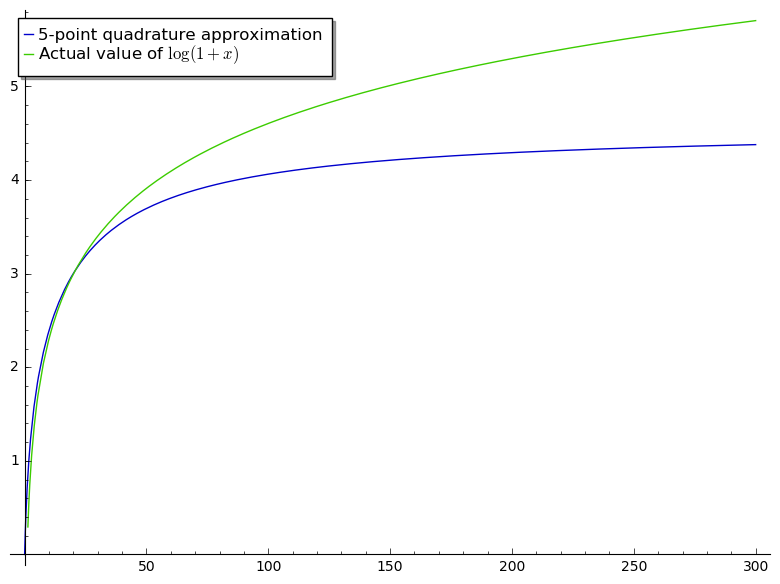
\includegraphics[width=.8\linewidth]{figures/StandardQuadrature.png}
%     \caption{Graph of $\log{(1+x)}$ and the approximation in equation \ref{eq:standardquadrature}}
%     \label{fig:standardquadrature}
% \end{figure}
\begin{figure}[!ht]
    \centering
	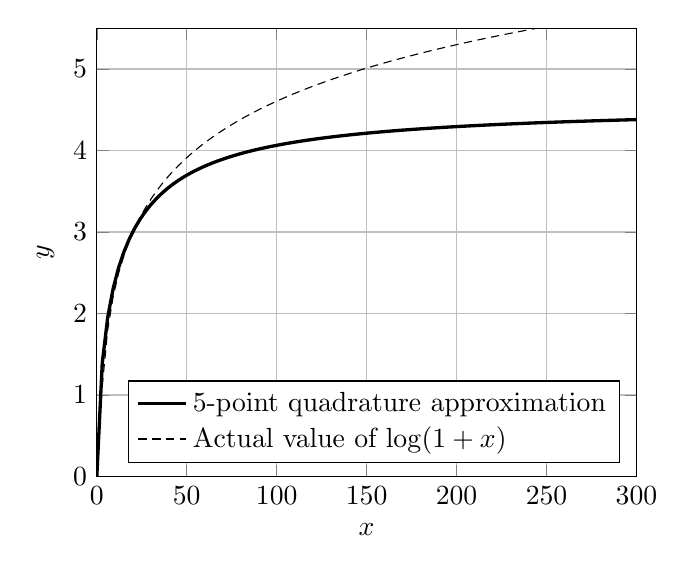
\begin{tikzpicture}
		\begin{axis}[
			% height=6cm, width=9cm,
			xmin=0, xmax=300,
			ymin=0, ymax=5.5, ytick={0,...,6},
			xlabel={$x$}, ylabel={$y$},
			grid=major,
			legend pos=south east,
			legend cell align=left,
		]
		\addplot[very thick, domain=0:300, samples=100]{1/30*(137*x^5 + 2310*x^4 + 9870*x^3 + 15120*x^2 + 7560*x)/(x^5 + 30*x^4 + 210*x^3 + 560*x^2 + 630*x + 252)};
		\addplot[densely dashed, domain=0:300, samples=100]{ln(x)};
		\legend{5-point quadrature approximation, Actual value of $\log(1+x)$}
		\end{axis}
	\end{tikzpicture}%
    \caption{Graph of $\log{(1+x)}$ and the approximation in Equation~\ref{eq:standardquadrature}}
    \label{fig:standardquadrature}
\end{figure}

As we only need accuracy for arguments $x \in [0, 255]$, we can scale the approximation by a constant factor $\alpha$ as follows:
\begin{align*}
  \log{(1+x)} &= \log{\left(\frac{\alpha + \alpha x}{\alpha}\right)}\\
  &= \log{(\alpha + \alpha x)} - \log{\alpha}\\
  &= \log{\left(\alpha+\frac{\alpha}{n}\right)} - \log{\alpha}\\
  &= \log{\left(\frac{\alpha n + \alpha}{n}\right)} - \log{\alpha}\\
  &= \int_{n}^{\alpha n + \alpha}{\frac{1}{x}\diff x} - \log{\alpha}
\end{align*}

Applying the five-point Gauss--Legendre quadrature rule with $\alpha = 1/20$ using SageMath 8.3, we arrive at the approximation:
\begin{align}\label{eq:scaledquadrature}
  \begin{split}
    &\log(1+x) \\
    &\approx \frac{137x^5 + 33185x^4 + 931370x^3 - 13403630x^2 - 289469315x - 713567363}
    {30(x^5 + 505x^4 + 42010x^3 + 923010x^2 + 5722005x + 8040501)} \\
    &+ \log{20}
  \end{split}
\end{align}

Figure~\ref{fig:scaledquadrature} is a graph of the absolute error of the scaled approximation and the exact value of $\log{(1+x)}$. Using SageMath 8.3, it was numerically determined that the maximum absolute error of this approximation in the range $x\in[0,255]$ is approximately $0.0103315865985758$, occurring at $x=255$. This is an improvement from the approximation in Equation~\ref{eq:standardquadrature}, which has a maximum absolute error of $1.19717868468392$, similarly occurring at $x=255$.

% \begin{figure}[h]
%     \centering
%     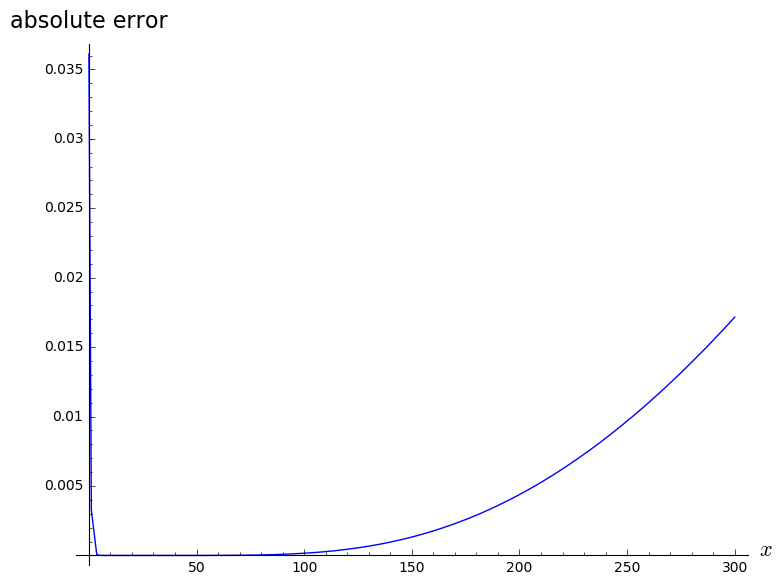
\includegraphics[width=.9\linewidth]{figures/ModifiedQuadratureAbsoluteError.png}
%     \caption{Graph of the absolute error of $\log{(1+x)}$ and the approximation in equation \ref{eq:scaledquadrature}}
%     \label{fig:scaledquadrature}
% \end{figure}
\begin{figure}[h]
    \centering
    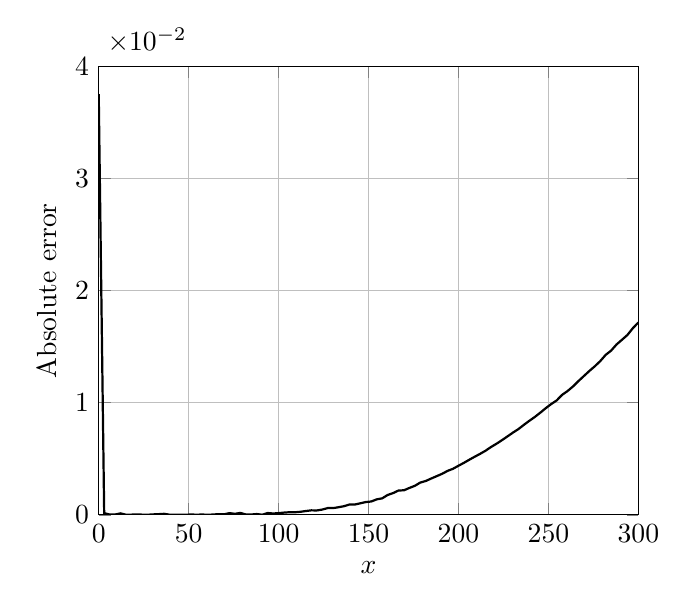
\begin{tikzpicture}
		\begin{axis}[
			% height=6cm, width=9cm,
			xmin=0, xmax=300,
			ymin=0, ymax=0.04,
			xlabel={$x$}, ylabel={Absolute error},
			grid=major,
			legend pos=south east,
			legend cell align=left,
			tick scale binop=\times,
		]
		\addplot[thick, domain=0:300, samples=100]{abs((1/30*(137*x^5 + 33185*x^4 + 931370*x^3 - 13403630*x^2 - 289469315*x - 713567363)/(x^5 + 505*x^4 + 42010*x^3 + 923010*x^2 + 5722005*x + 8040501))-ln((1/20)+(1/20)*x))};
		\end{axis}
	\end{tikzpicture}%
    \caption{Graph of the absolute error of $\log{(1+x)}$ and the approximation in Equation~\ref{eq:scaledquadrature}}
    \label{fig:scaledquadrature}
\end{figure}

\subsection{Approximation for $x^\gamma$}
\label{sec:approx-pwr}
To approximate $x^\gamma$ for any $\gamma \in \mathbb{R}$, we rewrite $x^\gamma$ as follows:
\begin{align*}
  x^\gamma = e^{\log{x^\gamma}} = e^{\gamma\log{x}}.
\end{align*}

This expression can then be approximated using the Maclaurin series expansion for $e^x$, which converges for all $x$.
\begin{align*}
  e^x &= \sum_{n=0}^{\infty}{\frac{x^n}{n!}}\\
  \Rightarrow \quad e^{\gamma\log{x}} &= \sum_{n=0}^{\infty}{\frac{(\gamma\log{x})^n}{n!}}
\end{align*}

As we already have an approximation for the natural logarithm, we can evaluate partial sums of the above infinite series to arrive at approximations for $x^\gamma$.
% \balancecolumns

\end{document}
